\chapter{Transfer Function Optimization Using Visibility-Weighted Saliency}
Volume visualization is an effective means of discovering meaningful features in volume data sets. Users can reveal the exterior and interior of structures by specifying opacity values for the features in transfer functions. Features can be intensity intervals in 1D transfer functions, rectangular or other shapes in 2D or higher-dimensional transfer functions.

\section{Introduction}
Volume visualization has proven to be an effective means of discovering meaningful features in volume data sets. By specifying appropriate opacity values for various features, the exterior and interior features can be simultaneously revealed in a semi-transparent manner.

%-------------------------------------------------------------------------
\section{Method}
In Chapter~\ref{visibility-weighted_saliency}, visibility-weighted saliency was proposed as a measure of visual saliency of features in volume rendered images, in order to assist users in choosing suitable viewpoints and designing effective transfer functions to visualize the features of interest. In this chapter, we describe a transfer function optimization approach based on the visibility-weighted saliency metric, which indicates the perceptual importance of voxels and the visibility of features in volume rendered images.

The approach described in Chapter~\ref{transfer_function_refinement} is an automated method of optimizing transfer functions, based on the intensity distribution of voxels in the volume data set. However, this approach does not take into account the spatial distribution of voxels and the viewpoint of the visualization. Visibility-weighted saliency, on the other hand, takes into account both of these two aspects. The visibility-weighted saliency consists of two component fields, i.e. saliency field and visiblity fields. Saliency fields are essentially difference of Gaussians, which include the information of local neighborhoods of voxels, and visibility fields are computed from opacity contribution of voxels to volume rendered images, which indicate viewpoint dependent occlusions of the voxels.

\subsection{Objective Function}
Users define target importance values for each feature defined in the transfer function domain.
Our approach adjusts the transfer function to match the visibility-weighted saliency with the user-defined target importance values.
Multiple saliency fields computed from different appearance attributes can be combined together in order to represent different aspects of the visual saliency of voxels.
In our implementation, brightness and saturation are used respectively to compute visibility-weighted saliency fields and define the weighted sum of the two sets of feature saliency as visibility-weighted feature saliency.
The objective function is defined as the root mean square of the differences of the visibility-weighted saliency and target importance of each feature.
\[ E=\sqrt{ \frac{\sum_{i=1}^{n} (W_{i}-t_{i})^{2}}{n} } 
\addtag \]
where \[ W_{F}=u_{1}W_{F}(O_{b},i,\sigma)+u_{2}W_{F}(O_{s},i,\sigma) \] is the visibility-weighted saliency of feature $ i $, as previously described in Section~\ref{weighted_feature_saliency}. $ t_{i} $ is the user-defined importance of feature $ i $. These user-defined importance values are normalized and they add up to 1, in other words, $ t_{i} \in [0.1] $ and $ \sum_{i=1}^{n} t_{i} = 1 $.

However, the visibility-weighted saliency $ W_{i} $ is not a variable that can be directed modified. Instead, $ W_{i} $ is a complicated function dependent on the opacity values of features, the spatial distribution of voxels and the viewpoint of the visualization.

A nucleon data set \cite{website:Voreen_datasets_2013} to demonstrate how the visibility-weighted saliency of features change when the feature opacity values (mapped to $ x, y and z $ axes) change.

\begin{figure}
\centering
	\begin{minipage}{.25\textwidth}
	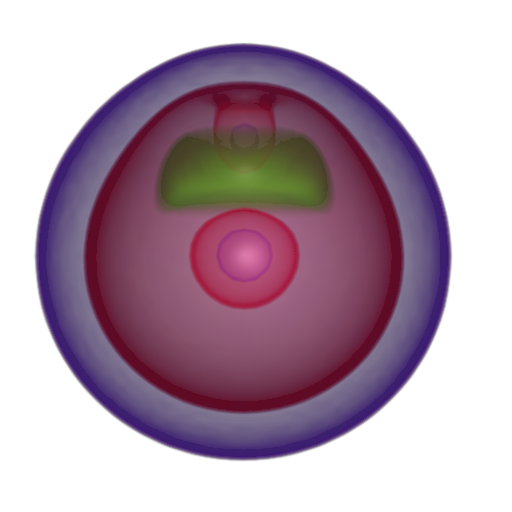
\includegraphics[width=1\linewidth]{images/nucleon_naive}
	\caption{a}	
	\end{minipage}~
	\begin{minipage}{.25\textwidth}
	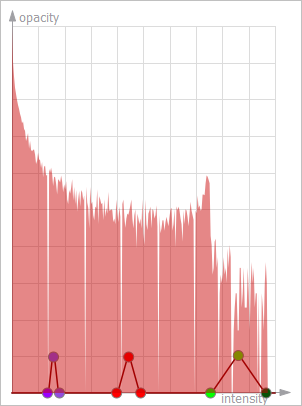
\includegraphics[width=1\linewidth]{images/tf_nucleon_naive}
	\caption{b}	
	\end{minipage}
	\label{fig:nucleon_naive}
\end{figure}



\subsection{Optimization Algorithm}


\subsection{Adaptive Step Size with Line Search}


\subsection{Adaptive Step Size with Parallel Search}

%-------------------------------------------------------------------------
\section{Results and Discussions}

%-------------------------------------------------------------------------
\section{Conclusions}
